%%%%%%%%%%%%%%%%%%%%%%%%%%%%%%%%%%%%%%%%%%%%%%%%%%%%%
% Primary document settings
%%%%%%%%%%%%%%%%%%%%%%%%%%%%%%%%%%%%%%%%%%%%%%%%%%%%%

\documentclass[aspectratio=169,12pt]{beamer}

\usepackage{ifxetex,ifluatex}
\ifnum 0\ifxetex 1\fi\ifluatex 1\fi=0 % if pdftex
  \usepackage[T1]{fontenc}
  \usepackage[utf8]{inputenc}
  \usepackage{textcomp} % provide euro and other symbols
\else % if luatex or xetex
  \usepackage{unicode-math}
  \defaultfontfeatures{Scale=MatchLowercase}
  \defaultfontfeatures[\rmfamily]{Ligatures=TeX,Scale=1}

\usepackage[
    backend=biber,
    natbib=true,
    style=authoryear-comp,
    %bibstyle=authoryear,
    %autocite=footnote,
    %style=authoryear,
    sorting=nyt,
    %sortlocale=de_DE,
    sortlocale=en_US,
    url=false,
    doi=true,
]{biblatex}


\usepackage{fancyqr}

%%%%%%%%%%%%%%%%%%%%%%%%%%%%%%%%%%%%%%%%%%%%%%%%%%%%%%%%%%%%%%
% Extra stuff for Rmarkdown to work (code blocks)
%%%%%%%%%%%%%%%%%%%%%%%%%%%%%%%%%%%%%%%%%%%%%%%%%%%%%%%%%%%%%%
\providecommand{\tightlist}{%
  \setlength{\itemsep}{2pt}\setlength{\parskip}{0pt}}

\usepackage{graphicx}
\makeatletter
\def\maxwidth{\ifdim\Gin@nat@width>\linewidth\linewidth\else\Gin@nat@width\fi}
\def\maxheight{\ifdim\Gin@nat@height>\textheight\textheight\else\Gin@nat@height\fi}
\makeatother
% Scale images if necessary, so that they will not overflow the page
% margins by default, and it is still possible to overwrite the defaults
% using explicit options in \includegraphics[width, height, ...]{}
\setkeys{Gin}{width=\maxwidth,height=\maxheight,keepaspectratio}
% Set default figure placement to htbp
\makeatletter
\def\fps@figure{htbp}
\makeatother

%%%%%%%%%%%%%%%%%%%%%%%%%%
% kableExtra stuff (tables)
%%%%%%%%%%%%%%%%%%%%%%%%%%
\usepackage{booktabs}
\usepackage{longtable}
\usepackage{array}
\usepackage{multirow}
\usepackage{xcolor}
\usepackage{wrapfig}
\usepackage{float}
\usepackage{colortbl}
\usepackage{pdflscape}
\usepackage{tabu}
\usepackage{threeparttable}
\usepackage{threeparttablex}
\usepackage[normalem]{ulem}
\usepackage{makecell}

%%%%%%%%%%%%%%%%%%%%%%%%%%
% Main document
%%%%%%%%%%%%%%%%%%%%%%%%%%

\usetheme[fira]{BIPS}
%\usetheme[german]{BIPS}  % for the German version
%\usetheme[fira]{BIPS} % English with the Fira font
%\usetheme[german,fira]{BIPS} % German with the Fira font

% Note that for the Fira font, you need to use
% XeLaTeX instead of pdfLaTeX. You can find this in
% most interfaces

\title{Journal Club\\
``Statistical Comparisons of Classifiers\\
Over Multiple Data Sets''\\
(Dem\v{s}ar, 2006)}
\subtitle{}
\author{Lukas Burk\inst{1,2}}
\date{2024-05-13}
\contactauthor{Lukas Burk}
\occasion{BioWimium}
\email{burk@leibniz-bips.de}
\institute{\textsuperscript{1}Leibniz Institute for Prevention Research
and Epidemiology -- BIPS \and \textsuperscript{2}LMU Munich}

%\author[Burk, Bender, Wright]% (optional, for multiple authors)
%{Lukas Burk\inst{1} \and Andreas Bender\inst{2,3} \and Marvin N. Wright\inst{1}}

%\institute%
%{
%  \inst{1}%
%  Leibniz Institute for Prevention Research and Epidemiology -- BIPS\\
%  \inst{2}%
%  LMU Munich\\
  %\and
%  \inst{3}%
%  Munich Center for Machine Learning (MCML)
%}

%%% Title Page
\setbeamertemplate{title page}{
	\usebeamercolor{title page}
	\begin{tikzpicture}
		\useasboundingbox (1,0) rectangle (\the\paperwidth,\the\paperheight);
		\node[font=\usebeamerfont{title}, color=BIPSBlue, text width=14cm, align=center] at (\paperwidth*.5,7) {\inserttitle} ;
		% \node[align=center, font=\usebeamerfont{subtitle}, color=BIPSBlue] at (\paperwidth*.5, 5.5) {\insertsubtitle};
		\node[align=center, font=\usebeamerfont{author}, color=BIPSBlue] at (\paperwidth*.5, 5) {\insertauthor};
		\node[align=center, font=\usebeamerfont{institute}, color=BIPSTextGray] at (\paperwidth*.5, 3) {\textsuperscript{1}Leibniz
Institute for Prevention Research and Epidemiology --
BIPS \\ \textsuperscript{2}LMU Munich};
		\node[align=center, font=\usebeamerfont{date}, color=BIPSTextGray] at (\paperwidth*.5, 1.5) {\insertdate};
		\node[align=center, font=\usebeamerfont{date}, color=BIPSTextGray] at (\paperwidth*.5, 1) {BioWimium};
	\end{tikzpicture}
}


%\author{Lukas Burk\inst{1} \and Andreas Bender\inst{2}\inst{3} \and Marvin N. Wright\inst{1}}
% Affiliations
%\institute[short]{\inst{1} Leibniz Institute for Prevention Research and Epidemiology - BIPS \\ \inst{2} LMU Munich \\ \inst{3} Munich Center for Machine Learning (MCML)}

\begin{document}
\addtocounter{framenumber}{-1}
\frame{\maketitle}

% \setcounter{framenumber}{1}


\begin{frame}{Dem\v{s}ar (2006)}
\phantomsection\label{demar-2006}
\begin{center}

\includegraphics[width=6.14in,height=0.7\textheight]{img/demsar_title.png}
\end{center}
\end{frame}

\begin{frame}{Context}
\phantomsection\label{context}
\begin{itemize}[<+->]
\tightlist
\item
  The year is 2006
\item
  Machine learning is happening
\item
  New algorithms published every 4 seconds
\item
  Authors compare their proposed method against SOTA\\
  \ldots using whichever means necessary, appropriate, valid.
\end{itemize}

\vfill
\pause

Comparing things is hard\textsuperscript{(citation needed)}
\end{frame}

\begin{frame}{Motivation and Setting}
\phantomsection\label{motivation-and-setting}
\begin{itemize}[<+->]
\tightlist
\item
  Goal: Compare \(k\) classification algorithms on \(N\) datasets
\item
  Common hypothesis:\\
  Does new algorithm perform better than established methods?
\item
  Comparing 2 classifiers on 1 dataset insufficient
\item
  Comparing multiple classifiers on multiple datasets: More difficult
\end{itemize}
\end{frame}

\begin{frame}{Setting}
\phantomsection\label{setting}
\begin{itemize}[<+->]
\tightlist
\item
  Evaluation produces score \(c_i^j\) for \(j\)-th algorithm on the
  \(i\)-th dataset
\item
  Scores: Accuracy, AUC or similar measure

  \begin{itemize}[<+->]
  \tightlist
  \item
    No recorded variance \(\Rightarrow\) no assumptions about resampling
    scheme
  \item
    Resampling for stability of scores only
  \end{itemize}
\item
  Algorithms evaluated on same datasets

  \begin{itemize}[<+->]
  \tightlist
  \item
    Sample size here ``Number of datasets in benchmark''
  \item
    \(\Rightarrow\) Datasets are independent, scores are not
  \end{itemize}
\end{itemize}
\end{frame}

\begin{frame}{Comparing 2 classifiers}
\phantomsection\label{comparing-2-classifiers}
\begin{itemize}
\tightlist
\item
  Paired t-test

  \begin{itemize}
  \tightlist
  \item
    Highest power when assumptions met
  \item
    Assumes commensurability of scores (questionable)
  \item
    Normality, outliers
  \end{itemize}
\end{itemize}

\pause

\begin{itemize}
\tightlist
\item
  Wilcoxon signed rank test

  \begin{itemize}
  \tightlist
  \item
    Only assumes commensurability of ranks
  \end{itemize}
\end{itemize}

\pause

\begin{itemize}
\tightlist
\item
  Sign test: Not even bothering with this one
\end{itemize}
\end{frame}

\begin{frame}{Comparing multiple classifiers}
\phantomsection\label{comparing-multiple-classifiers}
General scheme:

\begin{enumerate}
\tightlist
\item
  Perform global test to detect if any two algorithms differ at all
\item
  If (1) is signif., perform post-hoc test to detect which algorithms
  differ in particular
\end{enumerate}
\end{frame}

\begin{frame}{Global tests}
\phantomsection\label{global-tests}
\begin{block}{Repeated measures ANOVA}
\phantomsection\label{repeated-measures-anova}
\begin{itemize}
\tightlist
\item
  Assumes normality of scores
\item
  Assumes sphericity (\(\approx\) homoskedasticity)
\end{itemize}
\end{block}

\begin{block}{Friedman test}
\phantomsection\label{friedman-test}
\begin{itemize}
\tightlist
\item
  Non-parametric analogue to rmANOVA
\item
  Uses ranks from best (1) to worst (k), averages for ties
\item
  Test statistic \(Fr \sim F(k-1, (k-1)(N-1))\)
\end{itemize}
\end{block}
\end{frame}

\begin{frame}{Post-hoc tests}
\phantomsection\label{post-hoc-tests}
Choices of all \emph{pairwise} or \emph{one-to-many} tests\\
in either \emph{parametric} or \emph{nonparametric} flavors:

\vfill

\begin{table}
\centering
\begin{tabular}{lll}
\toprule
Type & All Pairwise & One-to-many\\
\midrule
Parametric & Tukey & Dunnet\\
Nonparametric & Nemenyi & Bonferroni-Dunn\\
\bottomrule
\end{tabular}
\end{table}
\end{frame}

\begin{frame}{Nemenyi}
\phantomsection\label{nemenyi}
Critical differences between two algorithms calculated as

\[CD = q_\alpha \sqrt{\frac{k(k+1)}{6N}}\]

\begin{itemize}
\tightlist
\item
  Critical values \(q_\alpha\) based on studentized range statistic
\item
  If difference in average ranks exceeds CD, they are signif. different
\end{itemize}
\end{frame}

\begin{frame}{Bonferroni-Dunn}
\phantomsection\label{bonferroni-dunn}
Test statistic (approx. normal) is calculated based on average ranks
(\(R\))\\
for algorithms \(i\) and \(j\)

\[z = \frac{(R_i - R_j)}{\sqrt{\frac{k(k+1)}{6N}}}\]

\begin{itemize}
\tightlist
\item
  Much greater power when comparing against baseline
\item
  Can use any other method to control for FWER (Bonferroni, Holm,
  Hochberg, \ldots)
\item
  Using Bonferroni-Dunn gives constant CD, easier to visualize
\end{itemize}
\end{frame}

\begin{frame}{Example 1}
\phantomsection\label{example-1}
Comparing 4 algorithms across 14 datasets

\begin{center}
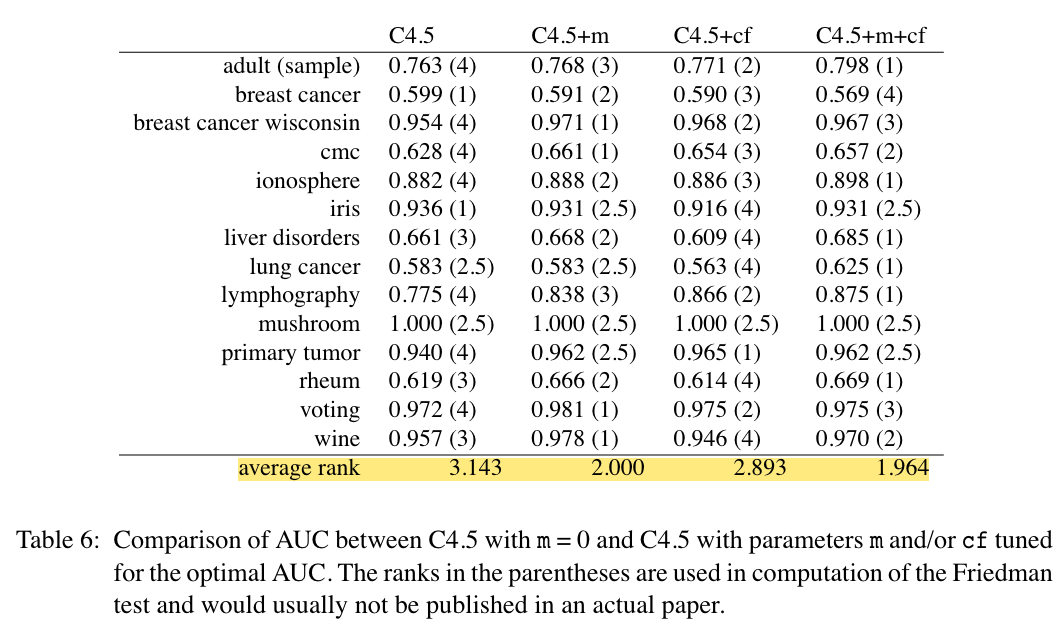
\includegraphics[width=3.52in,height=\textheight]{img/table6.png}
\end{center}
\end{frame}

\begin{frame}{Example 1: Result (Nemenyi, all pairwise)}
\phantomsection\label{example-1-result-nemenyi-all-pairwise}
\begin{itemize}
\tightlist
\item
  CD = \(2.569 \sqrt{\frac{4 \cdot 5}{6 \cdot 14}} = 1.25\) (for
  \(\alpha = 0.05\))

  \begin{itemize}
  \tightlist
  \item
    Difference between best and worst is already smaller
  \item
    Test not powerful enough
  \end{itemize}
\item
  CD = 1.12 (for \(\alpha = 0.1\)):

  \begin{itemize}
  \tightlist
  \item
    Conclude that C4.5 is worse than C4.5+m and C4.5+m+cf

    \begin{itemize}
    \tightlist
    \item
      Can't make statement about C4.5+cf
    \end{itemize}
  \end{itemize}
\end{itemize}
\end{frame}

\begin{frame}[fragile]{Example 1: Result (BD, one-to-many)}
\phantomsection\label{example-1-result-bd-one-to-many}
\begin{itemize}
\tightlist
\item
  Hypothesis: Does tuning \texttt{m} and/or \texttt{cf} help compared to
  baseline C4.5?
\item
  CD = 1.16
\end{itemize}

\[\begin{aligned}
\text{C4.5 vs. } & \text{C4.5+m+cf} & \rightarrow 3.143 − 1.964 = 1.179 > \color{green}{1.16} \\
\text{C4.5 vs. } & \text{C4.5+cf}   & \rightarrow 3.143 − 2.893 = 0.250 < \color{red}{1.16} \\
\text{C4.5 vs. } & \text{C4.5+m}    & \rightarrow 3.143 − 2.000 = 1.143 \approx \color{orange}{1.16}
\end{aligned}\]

\pause

\begin{itemize}
\tightlist
\item
  Conclude that tuning \texttt{m} helps, \texttt{cf} probably not
\end{itemize}
\end{frame}

\begin{frame}{Example 1: Critical Difference plots}
\phantomsection\label{example-1-critical-difference-plots}
All pairwise comparisons (top) vs.~baseline comparison (bottom)

\begin{center}
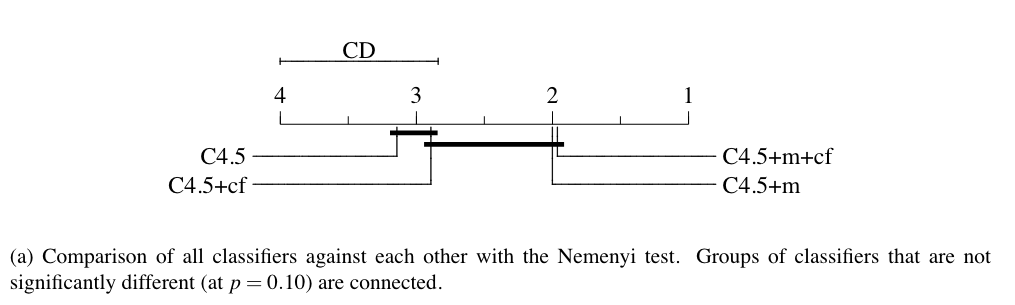
\includegraphics[width=3.38in,height=\textheight]{img/fig1-a.png}
\end{center}

\begin{center}
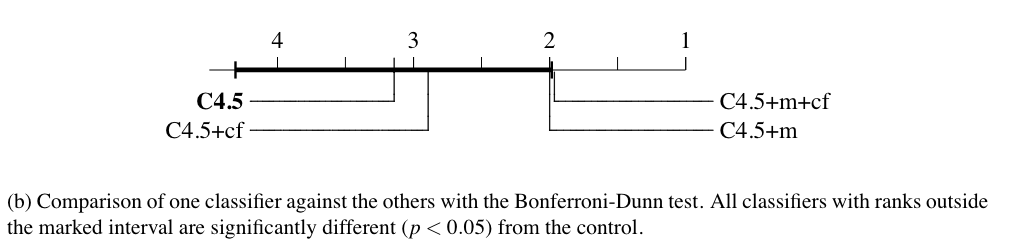
\includegraphics[width=3.36in,height=\textheight]{img/fig1-b.png}
\end{center}
\end{frame}

\begin{frame}{Empirical comparison of tests}
\phantomsection\label{empirical-comparison-of-tests}
\begin{itemize}[<+->]
\tightlist
\item
  Comparing various algorithms on 10 randomly drawn out of pool of 40
  real world datasets
\item
  No formal assessment of Type I / II error as correct test decision
  unclear
\item
  Measured performance of all algorithms on all datasets before
  experiment

  \begin{itemize}[<+->]
  \tightlist
  \item
    Introduce bias term \(k \geq 0\) to adjust difference between
    algorithms, affects selection of datasets
  \item
    \(k = 0\) corresponds to random choice of datasets
  \item
    Allows testing different hypothesis
  \end{itemize}
\item
  Calculate average p-values based on 1000 replicates
\end{itemize}
\end{frame}

\begin{frame}{Measures of reliability}
\phantomsection\label{measures-of-reliability}
\begin{enumerate}[<+->]
\tightlist
\item
  Variance of p values: \(R(p) = 1 - 2 \cdot \mathrm{Var}(p)\)
\item
  Measure based on Bouckaert (2004):
\end{enumerate}

\[R(e) = \sum_{1 \leq i < j \leq n} \frac{I(e_i = e_j)}{n(n-1)/2}\]
where \(e_i\) is outcome of \(i\)-th experiment out of \(n\) (1 if
accepted, 0 otherwise)

\begin{itemize}[<+->]
\tightlist
\item
  \(R(e) = 0.5\) if \# of rejected equals number of accepted
\item
  \(R(e) = 1\) if \# of rejected or accepted is 0 respectively
\item
  Will show low replicability if e.g.~p-values fluctuate closely around
  0.05
\end{itemize}
\end{frame}

\begin{frame}{Results}
\phantomsection\label{results}
\begin{center}
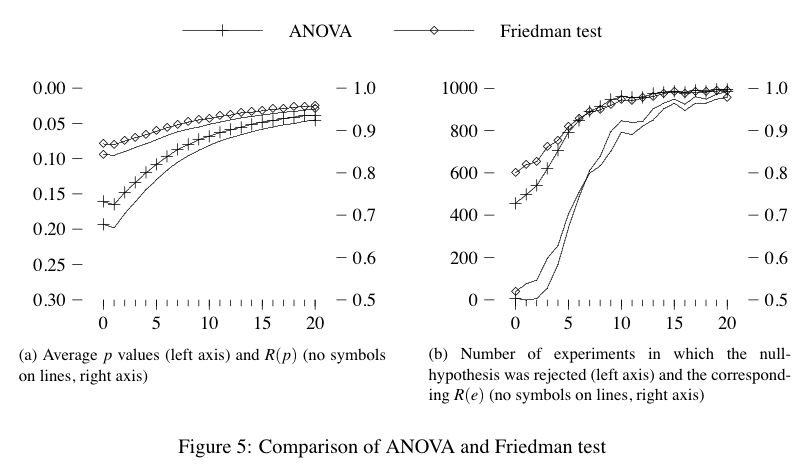
\includegraphics[width=0.95\textwidth,height=1.2\textheight]{img/fig5.png}
\end{center}
\end{frame}

\begin{frame}{Results}
\phantomsection\label{results-1}
\begin{center}
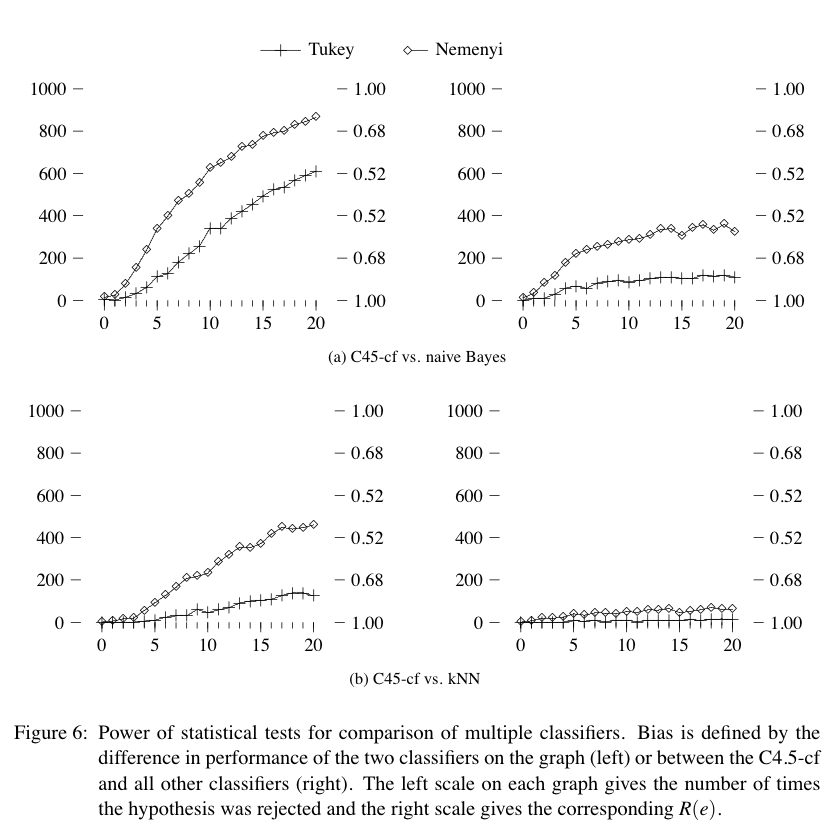
\includegraphics[width=2.76in,height=1\textheight]{img/fig6.png}
\end{center}
\end{frame}

\begin{frame}{Results}
\phantomsection\label{results-2}
\begin{center}
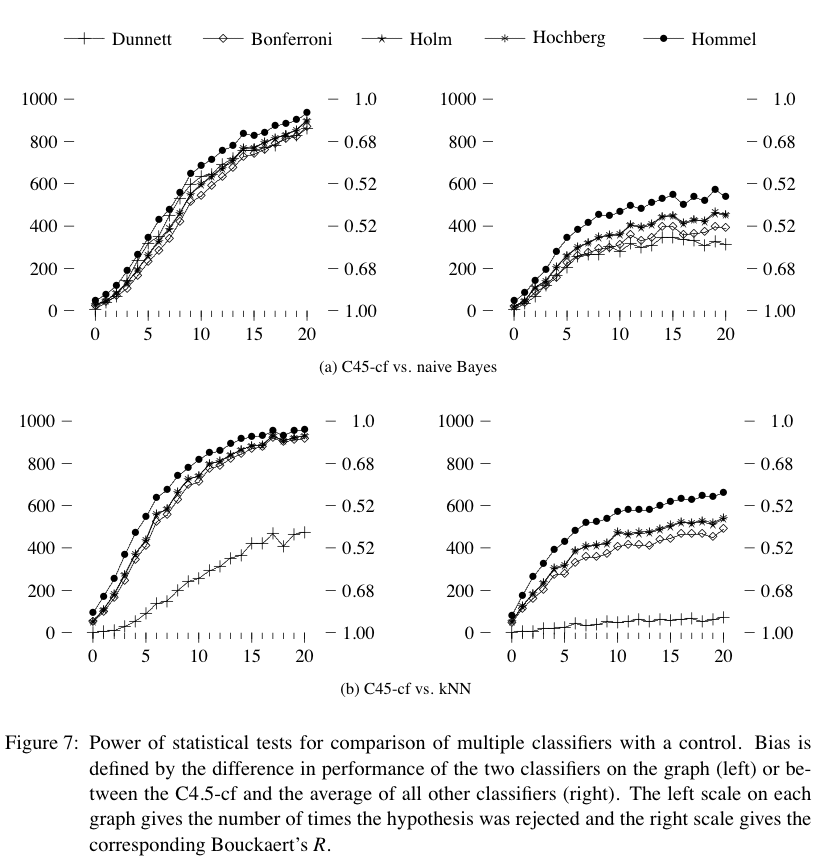
\includegraphics[width=2.76in,height=0.9\textheight]{img/fig7.png}
\end{center}
\end{frame}

\begin{frame}{Conclusion}
\phantomsection\label{conclusion}
\begin{itemize}
\tightlist
\item
  Nonparametric tests more likely to reject H0
\item
  Hints at violated assumptions of parametric tests
\end{itemize}

\vfill{} \pause

Nonparametric tests:

\begin{itemize}
\tightlist
\item
  Appropriate as they assume limited commensurability
\item
  Safer than parametric tests (assumptions)
\item
  Stronger than parametric tests here, especially for pairwise tests
\end{itemize}
\end{frame}

%%% Final slide with contact information
\thanksframe{Thank you for your attention!}

%%% bib?

\end{document}
